\chapter{Simulation}
This chapter discusses some simulation results, using a simple mathematical model to create a controller. First the mathematical model is discussed, after that the simulation results are discussed and compared with the internal Matlab sold.

\section{Trailer model}
The trailer model is illustrated in figure~\ref{fig:trailer model}, the left rectangle is the trailer and the right rectangle is the driver. The driver pulls the trailer forward. The driver is connect to the trailer via a single arm as illustrated in figure~\ref{fig:trailer model}. The control system can only change the speed in the Y and X axis. The goal of the control system is to get the trailer at a certain position and at a certain angle. Figure shows the trailer in a neutral position, so under an angle of 0 degrees.

\begin{figure}
	\centering
	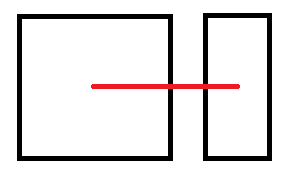
\includegraphics[width=0.5\textwidth]{trailer}
	\caption{trailer}
	\label{fig:trailer model}
\end{figure}

The mathematical model of the trailer is represented in equation~\ref{eq:trailer model} $u_x$ and $u_y$ are the inputs of the system and represent the speed in the Y and X direction. The angle is represented by $\theta$ , the distance between the driver and the trailer is represented by L. The position of the trailer is represented by $p_x$ and $p_y$.

\begin{equation}
	\begin{cases}
		\dot{p_x} = u_x + L sin \theta \cdot \dot{\theta} \\
		\dot{p_y} = u_y + L cos \theta \cdot \dot{\theta} \\
		\dot{\theta} = \frac{1}{L}(u_ycos \theta - u_x sin \theta)	
	\end{cases}
	\label{eq:trailer model}
\end{equation}

\section{A simple trailer example}
A simple way of measuring the performance of the library is to compared it to the alternatives. The nmpc-codegen library will be compared to, ForBes zerofrp2 the Matlab implementation of the panoc algorithm. And to the Matlab fmincon interior point,SQP and active set algorithms.

The simulation will contain four circular obstacles and the trailer will move from the lower left corner to the upper right corner. The state of the trailer will be represented by arrows, the starting point of the arrow is the position of the trailer. The angle of the arrow represents the positional angle of the trailer.

Figure~\ref{fig:path} contains the results of the simulation. The panoc algorithm chooses the lowest path while all three of the fmincon algorithms take the upper path. Both of these paths are valid solutions.


\begin{figure}[H]
	\centering
	\begin{subfigure}[b]{0.45\textwidth}
		\centering
		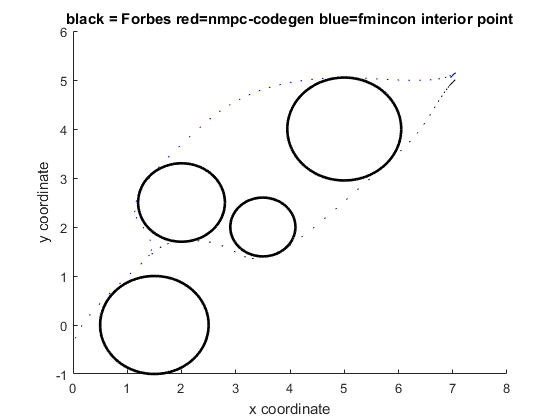
\includegraphics[width=1.2\textwidth]{compare_libs/path}
		\caption{path}
		\label{fig:path}
	\end{subfigure}
	
	\begin{subfigure}[b]{0.45\textwidth}
		\centering
		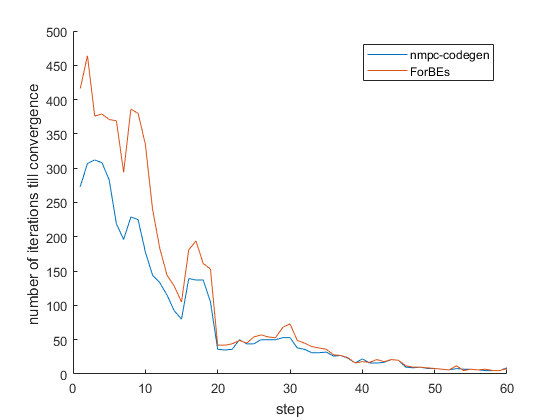
\includegraphics[width=1.2\textwidth]{compare_libs/iterations}
		\caption{iterations}
		\label{fig:iterations}
	\end{subfigure}
	\hfill
	\begin{subfigure}[b]{0.45\textwidth}
		\centering
		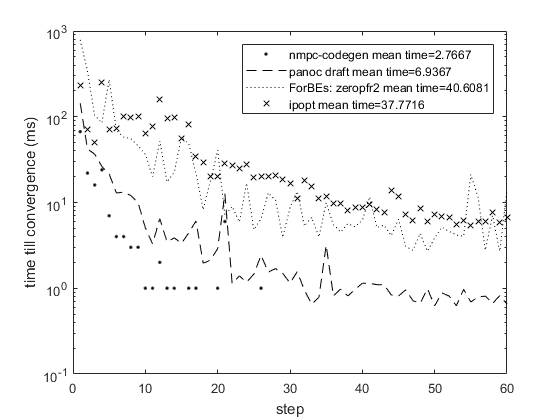
\includegraphics[width=1.2\textwidth]{compare_libs/timings}
		\caption{timings}
		\label{fig:timings}
	\end{subfigure}
	\caption{Schematic representation of the software}
\end{figure}